% %%%%%%%%%%%%%%%%%%%%%%%%%%%%%%%%%%%%%
% % Documentclass%{{{
% %%%%%%%%%%%%%%%%%%%%%%%%%%%%%%%%%%%%%
\documentclass[
	14pt,							% fontsize
	a4paper,						% paper-size
	landscape,						% paper-format: portrait & landscape
	titlepage,
	oneside,						% onesided layout for print; alternatively: twoside
	openany,						% openany: chapters start at the next empty page;
									% openright: chapters start at the next empty RIGHT page
	onecolumn,						% argument 'twocolumn' divides pages
	%flushbottom,					% flushbottom: makes all text pages the same height;
									% raggedbottom: height varies from page to page
	fleqn,							% equations are left-justified instead of being centered
	% leqno,							% equation numbers are on the left side
%
% %%%%%%%%%%%%%%%%%%%%%%%%%%%%%%%%%%%%%
% % KOMA
% %%%%%%%%%%%%%%%%%%%%%%%%%%%%%%%%%%%%%
%-- scrartcl/-book/-reprt: settings ---------------------------------------%{{{
	 headings=normal,				% fontsize for headings: small, normal, big
	 headsepline=true,				% true: horizontal line below the header
	 footsepline=false,				% true: horizontal line above the pagenumber
	 headinclude=false,				% true: add space between the top and the header
	 footinclude=false,				% true: add space between the bottom and the footnotes
	 twocolumn=false,				% true: split page in two columns
	 cleardoublepage=plain,			% like cleardoublepage, if a blank page is inserted it uses the style plain
	 bibliography=totoc,
	 listof=totoc,
	 toc=index,						% put stuff to toc
	 parskip=off,					% paragraph formatting. default: off; full+/%/-; half+/%/-
	 pagesize=pdftex				% paperhight is set via \pdfpagewidth and \pdfpageheight
%--------------------------------------------------------------------------%}}}
%
% %%%%%%%%%%%%%%%%%%%%%%%%%%%%%%%%%%%%%
% % Letters
% %%%%%%%%%%%%%%%%%%%%%%%%%%%%%%%%%%%%%
% dinbrief (german)
% akletter
% formlett
%%-- scrlttr2: settings ----------------------------------------------------%{{{
%	 %% Satzspiegel
%	 enlargefirstpage=on,			% Erste Seite anders
%	 pagenumber=headright,			% Seitenzahl oben mittig
%	 %
%	 %% Layout
%	 headsepline=on,				% Linie unter der Seitenzahl
%	 parskip=half,					% Abstand zwischen Absaetzen
%	 %
%	 %% Briefkopf und Anschrift
%	 fromalign=right,				% Plazierung des Briefkopfs
%	 fromphone=on,					% Telefonnummer im Absender
%	 fromrule=off,					% Linie im Absender (aftername, afteraddress)
%	 fromfax=off,					% Faxnummer
%	 fromemail=on,					% Emailadresse
%	 fromurl=off,					% Homepage
%	 fromlogo=off,					% Firmenlogo
%	 addrfield=on,					% Adressfeld fuer Fensterkuverts
%	 backaddress=off,				% ...und Absender im Fenster
%	 subject=beforeopening,			% Plazierung der Betreffzeile
%	 locfield=narrow,				% zusaetzliches Feld fuer Absender
%	 foldmarks=on,					% Faltmarken setzen
%	 numericaldate=off,				% Datum numerisch ausgeben
%	 refline=narrow,				% Geschaeftszeile im Satzspiegel
%	 %
%	 %% Formatierung
%	 draft=on				% Entwurfsmodus, als Formatierungshilfe -> on=ein, off=aus
%%--------------------------------------------------------------------------%}}}
%%-- newlfm: settings ------------------------------------------------------%{{{
	%sigleft,stdletter,orderfromtodate
							%% sigleft: signature to the left
							%% letter styles: stdletter, stdletternofrom, busletter, busletternofrom
							%% orderfromtodate: and date reordered to appear after the to-address
%%--------------------------------------------------------------------------%}}}
]{scrartcl}

\renewcommand{\arraystretch}{3.0}                      %% change space btw rows (default: 1.0)
% \setlength{\tabcolsep}{5pt}                            %% space btw columns (default value: 5pt)
%%%%%%%%%%%%%%%%%%%%%%%%%%%%%%%%%%%%%
% Title
%%%%%%%%%%%%%%%%%%%%%%%%%%%%%%%%%%%%%
% commands for \maketitle

% %%%%%%%%%%%%%%%%%%%%%%%%%%%%%%%%%%%%%
% Pagestyle %{{{
% %%%%%%%%%%%%%%%%%%%%%%%%%%%%%%%%%%%%%
\pagestyle{myheadings}

%	plain: 			The page number is in the foot and the head is empty. It is the default
%					page style for the 'article' and 'report' document.
%	empty: 			The head and foot are both empty. LaTeX still assigns each page a number,
%					but the number is not printed.
%	headings: 		The page number and other information, determined by the document
%					style, is put in the head; the foot is empty.
%	myheadings: 	Similar to the 'headings' page style, except you specify the "other
%					information" that goes in the head, using the \markboth and \markright commands
%					described below.
%}}}

% %%%%%%%%%%%%%%%%%%%%%%%%%%%%%%%%%%%%%
% Common-Packages %{{{
% %%%%%%%%%%%%%%%%%%%%%%%%%%%%%%%%%%%%%
\usepackage[ngerman]{babel}			% Neue Rechtschreibung
\usepackage[utf8]{inputenc}			% UTF-8
\usepackage[T1]{fontenc}			% Zur Darstellung von Umlauten
%
% %%%%%%%%%
% % some useful packages
% %%%%%%%%%
\usepackage[percent]{overpic}		% overlaying pic above another
\usepackage[printonlyused]{acronym} % printonlyused: only used acronyms are printed; other options: withpage
\usepackage{blindtext, xfrac}		% dummytext with '\blindtext'
\usepackage{charter}				% use the charter font for the document text
\usepackage{color}					% coloring eg. \textcolor{red}{... text}
\usepackage{enumitem}				% if you want to customize lists
\usepackage{eurosym}				% eurosymbol-package
\usepackage{graphicx}				% to include graphics
\usepackage{longtable}				% for long tables
\usepackage{pdfpages}				% inserting pdffiles
\usepackage{rotating}				% rotating tabulars
\usepackage{tabu}					% tabu-package
\usepackage{tabto}					% tabstops ('\tab') in list-environment
\usepackage{textcomp}				% additional characters
\usepackage{times}					% times new roman
\usepackage{url}					% for url
\usepackage{wrapfig}				% to get nice wrap of figures
\usepackage{xifthen}				% needed for citation-commands (see below!)
% \usepackage[left=0.5cm,top=0.5cm,bottom=1.0cm,includeheadfoot]{geometry}
%
% \usepackage[top=Bcm, bottom=Hcm, outer=Ccm, inner=Acm, heightrounded,
% marginparwidth=Ecm, marginparsep=Dcm]{geometry}
\usepackage[top=2cm,bottom=3cm, outer=15cm, inner=0.5cm, heightrounded,
marginparwidth=10cm, marginparsep=3.5cm]{geometry}
\usepackage[automark]{scrpage2}	% Should be set AFTER setting page geometry
									% automark, headsepline,
									% plainheadsepline, nouppercase
\usepackage{hyperref}
\hypersetup{pdftex,colorlinks=true,allcolors=blue}
\usepackage{hypcap}                                    % links should always anchor at the image not the caption.

% %%%%%%%%%
% % Math-Packages
% %%%%%%%%%
\usepackage{marginnote}
\usepackage{latexsym,amsfonts}
\usepackage{epsfig}
\usepackage{amsmath}
\usepackage{amssymb}
\usepackage{mathptmx}				% schrift times
\usepackage{array}					% texdoc array
\usepackage{bbm}
\usepackage{mathtools}				% http://ctan.org/pkg/mathtools
									% for 'case'-environment
%
% %%%%%%%%%
% Bibliography-Packages
% %%%%%%%%%
%\usepackage[numbers]{natbib}	% an extension to allow
							%% author-year citations along wih
							%% numerical citations. For more
							%% informations, texdoc Natbib
							%% options: numbers,super,sort&compress
							%% other packages: harvard, chicago etc.
%\usepackage{makeidx}		%% Single index (\makeindex); change makefile, if this is used
\usepackage{multind}		%% Make multiple indexes with multind; makefile
							%% sort both indexes eg. \makeindex{A}, \makeindex{B}
\usepackage[toc]{glossaries}		%% Making a nice glossary. Options: nonumberlist, toc
%
% %%%%%%%%%
% % Sidecaptions [optional]
% %%%%%%%%%
%\usepackage[demo]{graphicx}
%\usepackage{sidecap}
%\usepackage[outercaption]{sidecap}
%\usepackage[capbesideposition={top,outside},facing=yes,capbesidesep=quad]{floatrow}
%}}}

% %%%%%%%%%%%%%%%%%%%%%%%%%%%%%%%%%%%%%
% Silbentrennung und Rechtschreibung %{{{
% %%%%%%%%%%%%%%%%%%%%%%%%%%%%%%%%%%%%%
\tolerance=601						% Toleranzwert für die Silbentrennung
									% und den Abstand zw. Wörtern
\hyphenation{ }						% Ausnahmen für die automatische
									% Silbentrennung (jeweils durch
									% Leerzeichen getrennt eintragen)
%}}}

% %%%%%%%%%%%%%%%%%%%%%%%%%%%%%%%%%%%%%
% Headers, Indendation & Pagenumbering %{{{
% %%%%%%%%%%%%%%%%%%%%%%%%%%%%%%%%%%%%%
%
%%%%%%%%%
% % Headings
%%%%%%%%%
%\automark[section]{section}		% current section names at headline of every page
%\lehead{\author}				% overwriting even pages with the author's name
%
%%%%%%%%%
% % Indendation
%%%%%%%%%
%\setlength\parindent{0pt}		% globally suppress indentation
%\setcounter{secnumdepth}{0}	% unnumbers all headings (\parts, \subsections etc.), even when supposed to be numbered
%
%%%%%%%%%
% % Switch Pagenumbering on/off
%%%%%%%%%
\pagenumbering{arabic}			% set 'gobble' to switch off numbering. Other
								% options are: [Aa]lph, [Rr]oman, arabic
%}}}
%
% %%%%%%%%%%%%%%%%%%%%%%%%%%%%%%%%%%%%%
% Fonts %{{{
% %%%%%%%%%%%%%%%%%%%%%%%%%%%%%%%%%%%%%
% % Mit PDF-LaTeX
% % see: http://stackoverflow.com/a/877670
%\renewcommand{\familydefault}{\sfdefault} % This changes the default font family to sans-serif.
%
%If you want other fonts, try the following
%\setmainfont{Charis SIL}
%\setmainfont{URW Palladio L}
%\setmainfont{Linux Libertine O}
%\setmainfont{Gentium Book Basic}
%}}}

% %%%%%%%%%%%%%%%%%%%%%%%%%%%%%%%%%%%%%
% Commands %{{{
% %%%%%%%%%%%%%%%%%%%%%%%%%%%%%%%%%%%%%
%
%%%%%%%%%
% % Comments and indentation
%%%%%%%%%
\newcommand{\comment}[1]{\textcolor{red}{#1}}
% \renewcommand{\comment}[1]{}						% Comments: If both commands are used, the existing comments will be deleted
\newcommand{\ind}{\hspace{0.2in}}
\newcommand{\ftext}[1]{\text{\ind\footnotesize #1}}
\newcommand{\note}[1]{\marginnote{\em #1}}
%
%%%%%%%%%
% % Commands for Citation
%%%%%%%%%
%\AtBeginDocument{\renewcommand{\harvardand}{\&}}	% replaces and for & in harvard citation styles
%\AtBeginDocument{\renewcommand{\and}{\&}}			% replaces and for & in harvard citation styles
%
%%%%%%%%%
% % Commands for Letters etc
%%%%%%%%%
\newcommand{\myfirstname}{Jonas}
\newcommand{\mylastname}{Petong}
\newcommand{\mystreet}{Lohbergstr. 6}
\newcommand{\mypostcode}{44789}
\newcommand{\mycity}{Bochum}
\newcommand{\myphone}{0176 53347208}
\newcommand{\mymail}{jonas.petong@we.de}
%
%%%%%%%%%
% % Mathcommands
%%%%%%%%%
\newcommand{\sF}{\mathcal{F}}
\newcommand{\sH}{\mathcal{H}}
\newcommand{\sB}{\mathcal{B}}
\newcommand{\sD}{\mathcal{D}}
\newcommand{\sN}{\mathcal{N}}
\newcommand{\sO}{\mathcal{O}}
\newcommand{\mR}{\mathbb{R}}		% blackboard bold R
\newcommand{\mN}{\mathbb{N}}		% blackboard bold N
\newcommand{\mNO}{\mathbb{N}_0}
\newcommand{\mP}{\rm I\hspace{-0.7mm}P}
\newcommand{\mD}{\mathbb{D}}
\newcommand{\mDef}{
\overset{\text{\tiny def}}{=}}		% mathematical notion of “is defined as”.
\newcommand{\mF}{\mathbb{F}}
\newcommand{\mZ}{\mathbb{Z}}
\newcommand{\mQ}{\mathbb{Q}}
\newcommand{\bD}{\mathbf{D}}
\newcommand{\mE}{I\!\!E}
\newcommand{\si}{{(i)}}
\newcommand{\coloneqq}{\mathrel{\mathop:}=}
\newcommand{\eqqcolon}{=\mathrel{\mathop:}}
\newcommand{\norm}[1]{\left\lVert #1 \right\rVert}
\newcommand{\ip}[2]{\left< #1 , #2 \right>}
\newcommand{\Dom}{\text{Dom }}
\newcommand{\indicator}{\mathbf{1}}
\newcommand{\wh}[1]{\widehat{#1}}
% \newcommand{\cn}[1]{\citeasnoun{#1}}
%
%%%%%%%%%
% % Citations
%%%%%%%%%
% Requires \usepackage{xifthen} - Whatever-you-want-command:
% \newcommand{\cmdAlias}[2]{\defcitealias{#1}{#2}\kern-0.8ex\citetalias{#1}} %\kern-0.8ex removes a space
%
%% Alias mit zusätzlichem Argument (Seiten-, bzw. Kapitelangaben) --- xifthen-version plain
\newcommand{\cmdCite}[2][]{\citeauthor{#2}, \citeyear{#2}\ifthenelse{\isempty{#1}}{}{; #1}}
% cf. version with with braces
\newcommand{\cmdCiteBraces}[2][]{(\citeauthor{#2}, \citeyear{#2}\ifthenelse{\isempty{#1}}{}{; #1})}
\newcommand{\cmdCiteVgl}[2][]{(vgl. \citeauthor{#2}, \citeyear{#2}\ifthenelse{\isempty{#1}}{}{; #1})}
\newcommand{\cmdCiteAuth}[2][]{\citeauthor{#2}\ifthenelse{\isempty{#1}}{}{; #1}}
\newcommand{\cmdCiteYear}[2][]{\citeyear{#2}\ifthenelse{\isempty{#1}}{}{; #1}}
\newcommand{\cmdCiteTxt}[2][]{\citeauthor{#2} (\citeyear{#2}\ifthenelse{\isempty{#1}}{}{; #1})}
%}}}
\renewcommand{\arraystretch}{1.2}
%}}}
%%%%%%%%%%%%%%%%%%%%%%%%%%%%%%%%%%%%%
% % Title%{{{
%%%%%%%%%%%%%%%%%%%%%%%%%%%%%%%%%%%%%
\markright{Jonas Petong}
% commands for \maketitle
\title{Zusammenfassung}
\subtitle{WS 2013/14: Öko I}
\author{Jonas Petong}
\date{\today}

% press <CTRL+j>%}}}
\begin{document}
\maketitle
% \pagebreak

\section{Formeln}
\label{sec:formeln}
\begin{longtabu}to\textwidth{l@{\hspace{3cm}}c@{\hspace{3.0em}}p{0.6\textwidth}}
    Erwartungswert: $E(X)$ &%{{{
    \parbox[c]{0.5\textwidth}{
        \begin{align*}
            \sum X\cdot P(X=x)\\
            E(X)=\frac{1}{n}\sum^{n}_{i=1} X=\bar X
        \end{align*}
    }
    &$\begin{dcases}
        \sum^{J}_{j=1}\lbrack x_jf(x_j)\rbrack\text{~~für X diskret}\\
        \int^{\infty}_{-\infty}\lbrack xf(x)dx\rbrack\text{~~für X indiskret}
    \end{dcases}$\\
    %}}}
    Bedingter EW: $E(Y|X=x)$ &$\sum y\cdot P(Y=y|X=x)$\\
    Bedingte Verteilung: $P(Y=y|X=x)$ &$\dfrac{P(Y=y, X=x)}{P(X=x)}$\\
    Varianz: $Var(X)$ & $E\left(X-E(X)\right)^2$ & $\; E(X^2)-E(X)^2$ \\
    Standardabweichung: $SD(X)$&$\sqrt{Var(X)}$&$\sqrt{E(X^2)-E(X)^2}$\\
    Kovarianz:%{{{
    $cov(X,Y)$ & $E \left[ (X-EX)(Y-EY)\right] $&$ \; E(XY) - E(X)E(Y)$\\
    && $cov(X,Y)=0$, falls X u. Y unabh.\\
    && $cov(X,X)=E[(X-\mu x)^2]=\sigma^2x$ \\%}}}
    Korrelation: $corr(X,Y)$  &%{{{
    $\dfrac{cov(X,Y)}{\sqrt{Var(X)}\sqrt{Var(Y)}}$ & $1\leq corr(X,Y)\leq
    1$\\\\%}}}
    Schiefe: g & $\dfrac{E(X-EX)^3}{SD(X)^3}$&$g < 0: \text{linksschief}$; $g > 0: \text{rechtsschief}$\\%{{{%}}}
    Kurtosis: k  %{{{
    & $\dfrac{E(X-EX)^4}{SD(X)^4}$ & Schwere der Flanken einer Verteilung\\
    &&$\Rightarrow k < 3: \text{schwach gewölbt}$\\
&&$\Rightarrow k > 3: \text{stark gewölbt}$\\%}}}
    Koeffizient der Bestimmtheit: $R^2$%{{{
    \label{formula:R2}
    &$\dfrac{ESS}{TSS}$
    &$R^2$ ist der Anteil \emph{erklärter} Variation von $Y_i$ an der Gesamtregression ($\;\hat{=}\;1-\frac{SSR}{TSS}$)\\%}}}
    Das Angepasste $R^2$: $\bar{R}^2$&$1-\left( \frac{n-1}{n-k-1}\right)\frac{SSR}{TSS}$&Das \frqq adjustierte\flqq{} $R^2$ wird
    kleiner, da der Effekt der Regressoren auf das Modell herausgerechnet wird.\\
    Explained Sum of Squares: $ESS$
    &$\sum^{n}_{i=1} \left( \hat{Y}_i - \bar{\hat{Y}}\right)^2$&Die Summe der
    durch das Modell erklärten quadrierten Abweichung.\\
    Residual Sum of Squares: $SSR$
    & $\sum^{n}_{i=1} \hat{u}_i^2$&Summe der quadrierten Residuen.\\
    Total Sum of Squares: $TSS$
    &$\sum^{n}_{i=1} \left( Y_i - \bar Y \right)^2$&$\hat{=}\;ESS + SSR$\\
    Standardfehler der Regression: $SER$%{{{
    \label{formula:SER}&
    $\sqrt{\frac{1}{n-2}\sum \hat u_i^2 }$~~, mit $\sum\hat u_i^2 = SSR$&
    $\varnothing$-Größe der OLS Residuen\\
    &&$\Rightarrow SER$: Geschätzte SA von $u$\\
&&$\Rightarrow RMSE$: Geschätzte Standardabw. von $u$, ohne Korrektur der
    Freiheitsgrade.\\%}}}
    {\parbox[t]{0.5\textwidth}{
            F-Statistik bei Homoskedastie\\
            \begin{itemize}
                \item $k_{\text{unrestr}}=$ {\small Anzahl der Regressoren in der unrestr. Regression.}
                \item $q=${\small Anzahl der Restriktionen unter der Nullhypothese}
            \end{itemize}
        }
    }
    & $\frac{R^2_{\text{unrestr}} - R^2_{\text{restr}}/q} {1-R^2_{\text{unrestr}}/n-k_{\text{unrestr}}-1}$
    & Wenn die Fehler homoskedastisch sind, folgt die F-Statistik bei
    Homoskedastie einer $\chi^2_q/q$ -Verteilung in großen Stichproben. Die
    F-Statistik bei Homoskedastie ist historisch wichtig, aber nicht valide bei
    Heteroskedastie.\\
    &
\end{longtabu}


\pagebreak
\section{Beweise \& Funktionen}
\label{sec:derivations}
\begin{longtabu}to\textwidth{@{}l|cp{280pt}p{200pt}X}
	{\bfseries Verteilungsfunktion:}\\
	%.%%%%%%%%%%%%%%%%%%%%%%
	%.%%.Dichtefunktion %{{{
	%.%%%%%%%%%%%%%%%%%%%%%%
	Dichtefunktion für $X\sim N(0,1)$: $\phi(\frac{x-\mu}{\sigma})$
	&$\stackrel{\text{1. Abltg.}}{=}$&
	$
	\underbrace{\frac{\partial}{\partial x}\left( \frac{x-\mu}{\sigma}
	\right)}_{\text{innere Ableitung}} \cdot \underbrace{\Phi'\left( \frac{x-\mu}{\sigma}
	\right)}_{\text{äußere Ableitung}}
	$&
	Die erste Ableitung der Verteilungsfunktion F(x) wird als
	 Dichtefunktion von x bezeichnet: $\frac{1}{\sigma\sqrt{2\pi}}\cdot e^{-\frac{x^2}{2\sigma^2}}$\vspace{3ex}
	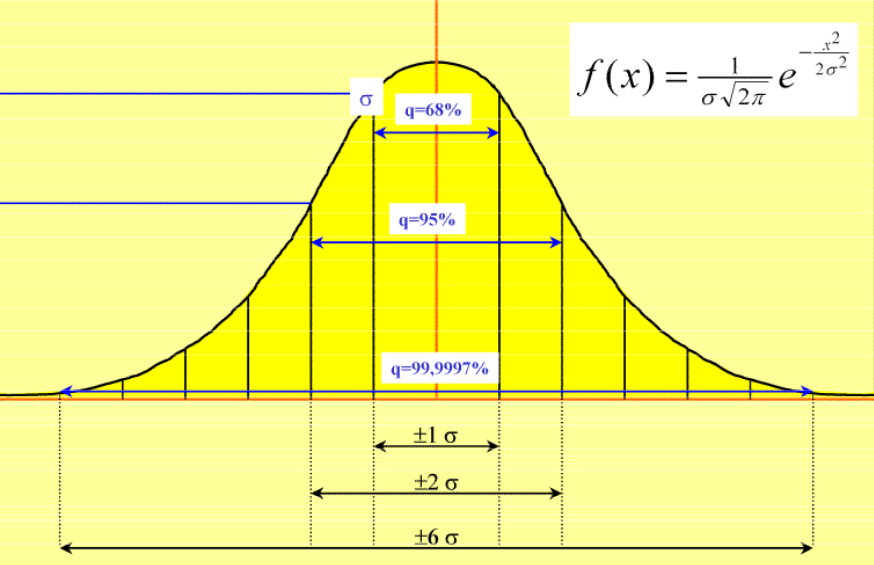
\includegraphics[width=28ex]{./sources/normvert_funkt_dichte}\\\\
 % \includegraphics*[width=15em,height=22ex]{./sources/normvert_funkt_dichte}\\
	%}}}

	{\bfseries Zu zeigen ist:}\\
	%.%%.a^2(Var(X)) %{{{
	%.%%%%%%%%%%%%%%%%%%%
	$Var(aX+b)=a^2Var(X)$&&$E\left(aX+\textcolor{red}{b} - \underbrace{E(aX+\textcolor{red}{b})}_{=aEX}\right)^2$&Die Konstante 'b' lässt sich herauskürzen\\%{{{%}}}%{{}}
	%.%%.Var(X)+Var(Y)+2cov(X,Y) %{{{
	%.%%%%%%%%%%%%%%%%%%%%%%%%%%%%%%%
	\\\\$Var(X+Y)=Var(X)+Var(Y)+2cov(X,Y)$&&$E\left(X+Y-E(X+Y)\right)^2$&$E(X+Y)=EX+EY$, aber\\
	&&&$Var(X+Y)\neq Var(X)+Var(Y)$\\
	&=&$E\underbrace{\left(X+Y -
	EX-EY\right)^2}_{\lbrack(X-EX)+(Y-EY)\rbrack^2}$\\
	&$\stackrel{\text{\tiny
	bin.~Form.}}{=}$&$(X-EX)^2+(Y-EY)^2+2\textcolor{blue}{E\mathbf\lbrack}(X-EX)(Y-EY)\textcolor{blue}{\mathbf\rbrack}$\\
	&=&$Var(X)+Var(Y)+2\cdot cov(X,Y)$
	%}}}
	%.%%.ac*cov(X,Y) %{{{
	%.%%%%%%%%%%%%%%%%%%%
	\\\\$cov(aX+b,cY+d)=ac\cdot cov(x,y)$&$\stackrel{\text{\tiny
	def}}{=}$&$E\lbrack\left(aX+\textcolor{red}{b}-E(aX+\textcolor{red}{b})\right)\left(cY+\textcolor{red}{d}-E(cY+\textcolor{red}{d}\right))\rbrack$\\
	&=&$E \lbrack a(X-EX) \cdot c(Y-EY) \rbrack $\\
	&=&$ac\underbrace{E(X-EX)(Y-EY)}_{cov(X,Y)}$
	%}}}
	%.%.Cov(X,Y) = 0 %{{{
	%.%%%%%%%%%%%%%%%%%%%
	\\\\
	$\underbrace{Cov(X,Y)=0}_{\text{wenn }X\bot Y \text{ und gemeinsam
	absolut stetig verteilt!}}$\vspace{10ex}
	&$\Rightarrow$&
	{$\!\begin{aligned} % http://tex.stackexchange.com/q/98482/16595 
				E(X,Y)=&\int^{\infty}_{-\infty}\int^{\infty}_{-\infty}xy\underbrace{f(x,y)}_{f_x(x)f_y(y)}dxdy\\
					&\int^{\infty}_{-\infty}\int^{\infty}_{-\infty}xf_x(x)dx\cdot yf_y(y)dy\\
	&=E(X)\;\cdot\;E(Y)
	\end{aligned}$}&
Da $Cov(X,Y)=\overbrace{E(XY)-EXEY}^{\text{Verschiebungssatz}}$ ist $Cov=0$, falls X u Y unabh (!)\\
	%}}}
\end{longtabu}


\pagebreak
\section{Verschiebungssätze}
\label{sec:verschiebungssatze}
\subsection{Varianz}
\label{sub:varianz}

\begin{align*}
	Var(X)&= E\bigl((X-E(X))^2\bigr)\\&
	= E\bigl(X^2 - 2XE(X) + E(X)^2\bigr)\\  &
	= E(X^2) - E\bigl(2XE(X)\bigr) + E\bigl(E(X)^2\bigr)\\&
	= E(X^2) - \underbrace{2E(X)E(X)}_{2E(X)^2} + E(X)^2\\&
	= E(X^2) - E(X)^2
\end{align*}\label{eq:versch_satz_1}
% subsection varianz (end)

\subsection{Kovarianz}
\label{sub:kovarianz}

\begin{align*}
	Cov(X,Y) &= {E}\left[ (X-EX)(Y-EY)\right]\\
			&=  {E}\bigl[(XY - X E(Y) - Y E(X) +  E(X) E(Y))\bigr]\\
   &= {E}(XY) - {E}(X) {E}(Y) \textcolor{red}{-{E}(Y) {E}(X) + {E}(X) {E}(Y)}\\
   &=  {E}(XY) - {E}(X) {E}(Y)
\end{align*} \label{eq:versch_satz_2}

% subsection kovarianz (end)


\pagebreak
\section{Herleitungen}
\label{sec:verschiebungssatze}
% \subsection{Schätzer der Varianz: $s_y^2$}
% \label{subsec:schatzer_der_varianz_von_y}
% % sub: schaetzer_der_varianz_von_y {{{ %

\begin{align*}
s^2_y&=\frac{1}{n-1}\sum^{n}_{i=1} \left(y_i - \bar
y\right)^2\\
\marginnote{da $y$ binomailverteilt, gilt:\\$y_i^2 \mDef y_i \mDef \bar y$ (!)}
&=\frac{1}{n-1}\sum^{n}_{i=1} \underbrace{ \left({y_i^2} - 2\bar{y}y_i +
\bar{y^2} \right)}_{y_i = \bar y}\\
&=\frac{1}{n-1}n \bar y -
\textcolor{red}{2}n \bar y^2 + \textcolor{red}{n \bar y^2}\\
&=\frac{n}{n-1}\left( \bar y - \bar y^2\right)\\
&=\frac{n\bar y}{n-1}\cdot (1 -
\bar y)\marginnote{entspr: $p\cdot(1-p)$}\\
\end{align*}
% subsection schatzer_der_varianz_von_y (end) %}}}


	\subsection{Unverzerrtheit des Schätzers $\beta_0$}
	\label{ssec:unbiasedness_beta_0}
% sssec %%% unbiasedness_beta_0 %{{{
Unter der Annahme des Regressionsmodells $y_i = \beta_ 0 + \beta_ 1 x_i +
u_i,\, i = 1, \ldots, n$ soll für den OLS-Schätzer $\hat\beta_0$ gelten:
$E(\hat\beta_0)=\beta_0$. Es sei $\hat\beta_1$ ein unverzerrter Schätzer für $\beta_1$.\\\\
Beachte:
\marginnote{somit
\begin{align*}
	\bar y &= \frac{1}{n}\sum^{n}_{i=1} (\beta_0 + \beta_1 x_i + u_i)\\
		&=\beta_0 + \beta_1 \bar x + \frac{1}{n}\sum^{n}_{i=1} u_i\\
\end{align*}
}

\begin{align*}
	y_i&=\beta_0 + \beta_1 x_i + u_i
\end{align*}\\

Beweis:
\begin{align*}
	E(\hat\beta_0)&=E(\bar y - \hat\beta_1\bar x)\\
	&=E(\underbrace{\beta_0 + \beta_1 \bar x +
\frac{1}{n}\sum^{n}_{i=1} u_i}_{\bar y} - \hat\beta_1 \bar x)\\
\marginnote{
	\begin{itemize}
\item 	$\bar x E(\beta_1 - \hat\beta_1) = 0$, da $\hat \beta_1$ unverzerrt,
\item $E[E(u_i|X=x_i)]=0$, nach LSA 1,\\
\item Da $\beta_0$ eine Konstante, ist $E\beta_0 = \beta_0$.
	\end{itemize}
}\\
%%%
&=E(\beta_0) + \underbrace{\comment{E[(\beta_1 - \hat\beta_1)\bar x]}}_{\bar x
E(\beta_1 - \hat\beta_1)} + \underbrace{\comment{\frac{1}{n}\sum^{n}_{i=1}
E(u_i)}}_{E[E(u_i|x_i)]}\\
%%%
E(\hat\beta_0)&=\beta_0
\end{align*}
% sssec %%% unbiasedness_beta_0 (end) %}}}


	\subsection{Unverzerrtheit des Schätzers $\beta_1$}
	\label{ssec:unbiasedness_beta_1}
% sssec %%% unbiasedness_beta_1 %{{{
Unter der Annahme des Regressionsmodells: $y_i = \beta_ 0 + \beta_ 1 x_i +
u_i,\, i = 1, \ldots, n$ soll für den OLS-Schätzer $\hat\beta_1$ gelten:
$E(\hat\beta_1)=\beta_1$\\\\

\begin{align*}
	\hat\beta_1-\beta_1&=\frac{\sum^{n}_{i=1} (x_i - \bar x)(y_i-\bar y_i)}{\sum^{n}_{i=1}
(x_i - \bar x)^2}-\beta_1
\end{align*}\\

Beweis:

\begin{align*}
	\hat\beta_1 - \beta_1&=\frac{
	\sum (x_i - \bar x)
(\overbrace{(\comment{\beta_0}+\beta_1 x_i +
u_i)}^{y_i}-\overbrace{(\comment{\beta_0}+\beta_1 \bar x + \bar u)}^{\bar y})
} {\sum (x_i-\bar x)^2}-\beta_1\marginnote{es gilt: $\bar y = \frac{1}{n} \sum y_i = \beta_0 + \beta_1 \bar x + \bar u$}\\
%%%
&=\frac{\sum (x_i - \bar x)\left( \beta_1(x_i - \bar x) + \comment{(u_i -\bar u)} \right)}{\sum (x_i - \bar x)^2} -\beta_1
\marginnote{
		$(u_i - \bar u) = 0\text{, da:~} u_i - \overbrace{\frac{1}{n}\sum u_i}^{= \bar u}$\\ %= u_i(\underbrace{1-\frac{1}{n}\sum 1}_{=0})$\\
		nach LSA 1 ist $E(u|X=x_i)=0$
}\\
%%%
&=\underbrace{\beta_1 \cdot \frac{\sum (x_i - \bar x)^2}{\sum (x_i - \bar x)^2} - \beta_1 }_{=0}
\end{align*}
Hieraus folgt, dass $$E(\hat\beta_1) - \beta_1 = 0$$
\marginnote{
\noindent
Also impliziert die KQ Annahme \#1, dass $E(\hat\beta_1) = \beta_1$. Das heißt,
$\hat\beta_1$ {\itshape ist ein unverzerrter Schätzer für} $\beta_1$
}

% sssec %%% unbiasedness_beta_1 (end) %}}}


\subsection{Binäre Variable \#1}
\label{ssec:binare_variable_1}
% subsect %%% binare_variable %{{{
Übung 3.3: Betrachten Sie die Regression $Y_i = \beta_0 + \beta_1 X_i + u_i$ , wobei $X_i$
eine binäre Variable ist. Bezeichne mit $\bar y_0$ bzw. $\bar y_1$ das Stichproben-Mittel
über alle Beobachtungen mit $X = 0$ bzw. $X = 1$.\\

Behauptung:
\begin{align*}
\hat\beta_1 = \bar y_1 - \bar y_0,\, \hat\beta_0 = \bar y_0 \text{ und }
\hat\beta_0 +\hat\beta_1&=\bar y_1\marginnote{$n_0 =$ Anzahl der Beobachtungen mit $x=0$\\$n_1=$Anzahl der Beobachtungen mit $x=1$}\\
\end{align*}

Beachte im Folgenden:
\begin{align}
	\sum^{n}_{i=1} x_i &= n_1\\
	\bar x &\stackrel{1)}{=} \frac{n_1}{n}\\
	\sum^{n}_{i=1} y_i&=\frac{1}{n_1} \sum^{n}_{i=1} x_i y_i=\bar y_1
\end{align}

\begin{align}
	\begin{split}
		\sum^{n}_{i=1} (x_i - \bar x)^2 &= \sum^{n}_{i=1} (x_i^2 - 2x_i \bar x + \bar x^2)\\
					&=(\sum^{n}_{i=1} x_i) - n\bar x^2 \\
				 &\stackrel{1)2)}{=}n_1 -n \left( \frac{n_1}{n} \right)^2\\
		   &=n_1 - \textcolor{blue}{n}\frac{n_1^2}{\textcolor{blue}{n}^2}=\frac{n_1 n - n_1^2}{n}\\
	&= \frac{n_1(n-n_1)}{n}\\
 &=\frac{n_1\cdot n_0}{n}=0\\
	\end{split}\marginnote{$x_i \mDef \bar x$ und $x_i^2 \mDef x_i$}
\end{align}

\begin{align}
	\begin{split}
		\bar y_1 +  \bar y_0 &=  y_i\\
		n_1 \bar y_1 + n_0 \bar y_0 &= \sum^{n}_{i=1} y_i
		\marginnote{dividiert durch $n$:\\$\bar y = \frac{n_1}{n} \bar y_1 +
		\frac{n_0}{n}\bar y_0$}
	\end{split}
\end{align}

Damit:

\begin{align}
	\hat\beta_1&=\frac{\sum (x_i - \bar x)(y_i - \bar y)}{\sum^{n}_{i=1} (x_i - \bar x)^2}
\end{align}

\begin{align*}
	&=\frac{\sum x_i(y_i-\bar y)-\overbrace{\comment{\bar x(y_i-\bar
y)}}^{=0}}{\sum (x_i - \bar x)^2}
\marginnote{
	es gilt $\sum (x_i - \bar x)^2\stackrel{4)}{=} \frac{n_1 n_0}{n} $
}\\
%%%
&\stackrel{1)4)}{=}\frac{\sum x_iy_i -{n_1}\cdot\bar y}{\left(
\frac{n_1 n_0}{n}
\right)}\\
%%%
&\stackrel{3)}{=}\frac{\textcolor{red}{n_1}\bar {y_1} -
\textcolor{red}{n_1}\bar y}{\left( \frac{\textcolor{red}{n_1} n_0}{n} \right)}\\
%%%
&=\frac{n}{n_0}\left( \bar y_1 - \bar y \right)
\stackrel{5)}{=}\frac{n}{n_0}\left( \bar y_1 - \left(\frac{n_1}{n}\bar y_1 + \frac{n_0}{n}\bar y_0
\right) \right)\\
%%%
&=\frac{n}{n_0}\left( \textcolor{blue}{\bar y_1} - \frac{n_1}{n}\textcolor{blue}{\bar y_1} - \frac{n_0}{n}\bar y_0 \right)\\
%%%
&=\textcolor{blue}{\bar y_1} (\frac{n}{n_0}-\frac{\comment{n}\cdot
n_1}{n_0\cdot \comment{n}})-\bar y_0\frac{\comment{n}\cdot n_0}{n_0 \cdot
\comment{n}}\marginnote{da binomial: $n - n_1 = n_0$}\\
%%%
&=\bar y_1 \frac{n_0}{n_0} - \bar y_0 \frac{n_0}{n_0}\\
%%%
&=\bar y_1 -\bar y_0
\end{align*}

 Daher:
\begin{align*}
\hat\beta_0 &=\bar y - \hat\beta_1 \bar x\\
			&\stackrel{2)5)6)}{=\frac{n_1}{n}}\bar y_1 + \frac{n_0}{n}\bar y_0 -
	\left( \bar y_1 - \bar y_0 \right)\frac{n_1}{n}\\
	&=\frac{n_0 + n_1}{n}\bar y_0 \\
	&=\bar y_0
 \end{align*}
\newline

% subsect %%% binare_variable (end) %}}}


\subsection{Binäre Variable \#2 - Umkehrung der Vorzeichen}
\label{ssec:binare_variable_2}
% subsect %%% binare_variable %{{{
\setcounter{equation}{0}
Übung 4.5: Bestimmung des $R^2$ sowie $SER$ (siehe \nameref{formula:SER})
einer binären Regression, bei Umkehrung der Dummy-Variable. Regression vorher
(1) und jetzt (2):

\begin{align}
	& \widehat{\text{Lohn}_i} = \beta_0 + \beta_1 \times \text{Mann}_i + u_i \label{eq:lohn_mann}
\end{align}

\begin{align}
	\begin{split}
		\widehat{\text{Lohn}_i} &= \gamma_0 + \gamma_1 \times \text{Frau}_i + v_i \label{eq:lohn_frau}\\
		& = \gamma_0 + \gamma_1 (1-\text{Mann}_i) + v_i\\
		& = \underbrace{\gamma_0 + \gamma_1}_{\hat{=}\beta_0} \underbrace{- \gamma_1}_{\hat{=}\beta_1} \times\text{Mann}_i + v_i
	\end{split}
\end{align}\\

hieraus folgt:

\begin{align}
	\begin{cases}
		\beta_{0}&=\gamma_0 + \gamma_1\\
	\textcolor{blue}{\beta_1}&\textcolor{blue}{=-\gamma_1}
	\end{cases}
	\text{~und~}
	\begin{cases}
		\gamma_0&=\beta_0 + \textcolor{blue}{\beta_1}\\
	\gamma_1&= -\beta_1
	\end{cases}
\end{align}

Wegen Beziehung geschätzter Koeffizienten gilt: $\hat{u}_i=\hat{v}_i$
und es ergibt sich\ldots

\begin{align*}
	\begin{rcases}
		SSR&=\sum^{n}_{i=1} \hat{u_i}^2\\
		SER&=\sqrt{\frac{SSR}{n-1}} \\
	\end{rcases}
	\text{bleiben unverändert, und somit auch $R^2$ gleich.}
	\marginnote{Beachte: $R^2\mDef 1- \frac{SSR}{TSS}$}
\end{align*}


% subsect %%% binare_variable (end) %}}}


\subsection{Binäre Variable \#3 - Standardfehler unter Homo- und Heteroskedastie}
\label{ssec:binare_variable_3}
% subsect %%% binare_variable %{{{
Vorl. 4-24: Standardfehler eines binären Regressors\\

\noindent
{\bfseries Standardfehler falls Verteilung Homoskedastisch:}\\
$\hat{=}$ Gleiche Gruppenvarianzen
\begin{align*}
	SE = \sqrt{\frac{s_s^2}{n_s}+\frac{s_l^2}{n_l}}\marginnote{mit $s_i^2=SER_i$ (Stichproben-Standardabweichung)}
\end{align*}
{\bfseries Standardfehler unter Heteroskedastie:}\\
$\hat{=}$ Ungleiche Gruppenvarianzen
\begin{align*}
SE = s_p\sqrt{\frac{1}{n_s}+\frac{1}{n_l}}\marginnote{$s_p = $\frqq gepoolter\flqq{} Schätzer\\von  $\sigma^2$  sofern $ \sigma^2_l = \sigma^2_l$}
\end{align*}

% subsect %%% binare_variable (end) %}}}



\pagebreak
\section{Ordinary Least Squares (OLS)}
\label{sec:ordinary_least_squares_ols}
% subsect %%% kleinster_quadrate_schatzer %{{{

{\itshape Der OLS Schätzer minimiert die durchschnittlichen quadrierten Abweichungen zwischen den wahren Werten von $y_i$ und dem geschätzten Wert (auf der Regressionsgerade).}\\\\
\subsection{Least Square Assumptions (LSA)}
\label{subsect:lsa}
% subsect %%% least_square_assumptions %{{{

\begin{enumerate}
	\item Die bedingte Verteilung von $u$ gegeben $X$ hat einen Mittelwert von null,
		das heißt, $E (u|X = x) = 0.$
		Dies impliziert, dass $\hat\beta_1$ unverzerrt ist (siehe Herleitung
		\ref{ssec:unbiasedness_beta_1}).
	\item $(X_i, Y_i ), i = 1,..., n$, sind gemeinsam \emph {identically and
		independently distributed (i.i.d)} und liefern
		damit die Stichprobenverteilung von $\hat\beta_0$ und $\hat\beta_1$.
		Dies gilt sofern $X$, $Y$ zufällig gezogen wurden.
	\item Größere Ausreißer von $X$ oder $Y$ sind selten:\\
		$E(X^4)<\infty,\;E(Y^4)<\infty$
		\begin{enumerate}
			\item 		 Technisch, $X$ und $Y$ haben endliche vierte Momente
			\item		 Ausreißer können zu bedeutungslosen Ergebnissen von $\hat\beta_1$ führen
		\end{enumerate}
		% \hline
	\item $u$ ist homoskedastisch% / Keine perfekte Mutikollinearität.
		\marginnote{
			Die Annahmen 4 und 5 sind restriktiver und für die Praxis weniger relevant als LSA eins bis drei.
		}
	\item $u$ ist $N(0, \sigma^2 )$ verteilt.
\end{enumerate}

% subsect %%% kq_annahmen (end) %}}}

\subsection{Minimierungsproblem: Aus der Vorlesung (3-11)}
\label{subsect:aus_der_vorlesung}
% subsect %%% aus_der_vorlesung %{{{

Zeigen Sie, dass der Kleinste-Quadrate Schätzer $\hat\beta$ dem
Stichproben-Mittelwert entspricht. Betrachte hierzu das
Regressionsmodell: $y_i = \beta + u_i$,\enskip\enskip $i=1,\ldots,n$\\

Dem OLS-Schätzer geht die Frage voraus, wie sich $\beta_0$ und $\beta_1$ aus
den Daten schätzen lassen. Da $\bar y$ der Kleinste Quadrate Schätzer für
$\mu_y$ ist, löst $\bar y$: 
$$\underset{m}{min} \sum^{n}_{i=1}\left( y_i - m \right)^2$$

Demgegenüber steht der OLS-Schätzer, dieser löst:
$$\underset{b_0,\,b_1}{min} \sum^{n}_{i=1}\left[ y_i - (b_0 +b_1x_i)
\right]^2$$\\

\begin{align*}
	\text{Bedingung erster Ordnung:}\\
	0&\overset{!}{=}\frac{\partial}{\partial b_1} \sum^{n}_{i=1}
	\left[ y_i - b_1xi \right]^2\\
	&=\sum^{n}_{i=1} x_i\cdot2 \left[ y_i - b_1 x_i
\right]\marginnote{Innere Ableitung$\,\times\,$Äußere Ableitung}\\
&=\textcolor{red}{2} \sum^{n}_{i=1} x_iy_i -\textcolor{red}{2}b_1 \sum^{n}_{i=1} x_i^2\\
b_1&=\hat\beta_1=\dfrac{\sum^{n}_{i=1} x_iy_i}{\sum^{n}_{i=1} x_i^2}
\marginnote{$\hat\beta_1=\frac{\sum^{n}_{i=1} (x_i - \bar x)(y_i - \bar y)}{\sum^{n}_{i=1} (x_i-\bar x)^2}$}\\
\hat\beta_0 &= \bar y - \bar x \hat\beta_1
	\end{align*}

Das Modell lässt sich umschreiben als: $y_i=\beta_1 \cdot
\underbrace{x_i}_{x_i=1} + u_i.$
Eingesetzt in die Formel: $$\hat\beta_1= \dfrac{\sum^{n}_{i=1} 1\cdot y_i}{\sum^{n}_{i=1} 1^2}=\dfrac{1}{n} \sum^{n}_{i=1} y_i
\marginnote{Stichprobenmittelwert der Beobachtungen $y_i$}$$

	% subsect %%% aus_der_vorlesung (end) %}}}

\subsection{Omitted Variable Bias}
\label{sec:omitted_variable_bias}
% subsect %%% omitted_variable_bias %{{{


Als \emph{omitted variable bias} wird die Verzerrung des LS-Schätzers beschrieben,
welche als Folge einer ausgelassenen Variable auftritt. Damit eine
Variable \emph{Z} als \emph{omitted variable} bezeichnet wird, müssen
die folgenden Voraussetzungen eintreffen. Sie \ldots

\begin{itemize}
	\item ist eine Determinante von $Y$ (und übt somit einen Einfluss auf sie aus) {\bfseries und}
	\item korreliert mit dem Regressor $X$, d.h. $Corr(Z,X) \neq{0}$
\end{itemize}

wenn beide Bedingungen erfüllt sind, dann ist der LS-Schätzer $(\hat \beta_1)$ verzerrt! Es gilt somit:

\begin{align*}
	\hat \beta_1 \overset{P}{\rightarrow} \beta_1 + \left(
	\frac{\sigma_u}{\sigma_x} \right) \rho_{x_u}\text{~mit~} \rho_{x_u} \neq 0
\end{align*}
%}}}

\subsection{Gauß-Markov Theorem}
\label{sec:gauss_markov_theorem}
% subsect %%% gauss_markov_theorem %{{{
Unter den LSA 1--4 hat $\hat\beta_1$ die kleinste Varianz unter
allen linearen bedingt unverzerrten Schätzern (Schätzer, die lineare
Funktionen von $Y_1, \ldots, Y_n$ sind).
\begin{align*}
	\hat\beta_1 - \beta_1 &= \frac{\sum^{n}_{i=1} (x_i - \bar x)u_i}{\sum^{n}_{i=1} (x_i - \bar x)^2}
&=\sum^{n}_{i=1} w_i u_i\marginnote{mit $w_i=\frac{ (x_i - \bar x)}{\sum^{n}_{i=1} (x_i - \bar x)^2}$}
\end{align*}
Das G-M Theorem sagt, dass unter allen möglichen \{$w_i$\}, die KQ
Gewichte die kleinste $Var(\hat\beta_1)$ ergeben.\marginnote{Folie 4-40}
%}}}

\subsection{Multikollinearität}
\label{sec:multikollinearitat}
% subsect %%% multikollinearitat %{{{

\textbf{Perfekte Multikollinearität} liegt vor, wenn einer der Regressoren eine exakte
lineare Funktion der anderen Regressoren ist und resultiert in der Regel aus
einem Fehler in der Wahl der Regressoren, oder aus seltsamen Daten. Die Lösung
für perfekte Multikollinearität ist es, die Liste der Regressoren so zu
modifizieren, dass nicht länger perfekte Multikollinearität vorliegt.\\

\textbf{Imperfekte Multikollinearität} tritt auf, wenn zwei oder mehr
Regressoren sehr hoch korreliert sind, die Korrelation jedoch nicht genau ±1
ist. Imperfekte Multikollinearität führt also typischerweise zu großen
Standardfehlern für einen oder mehrere der Koeffizienten.\\

Für die Schätzung der OLS muss, zusätzlich zu den LSA 1-3, die Bedingung erfüllt
sein, dass \emph{keine Perfekte Multikollinearität} vorliegt.
% subsect %%% multikollinearitat (end) %}}}

\subsection{Interne \& Externe Validität}
\label{sec:interne_&_externe_validitat}
% subsect %%% interne_&_externe_validitat %{{{

{\bfseries Externe Validität:} die statistische Inferenz kann hin zu anderen
Populationen/Situationen verallgemeinert werden, wobei die “Situationen” sich
auf etwa die rechtliche, politische, zeitliche oder physische Umgebung
beziehen.\\\\
{\bfseries Interne Validität:} die statistische Inferenz bezüglich kausaler Effekte ist für
die betrachtete Population valide (“gute Statistik”).\\
Fünf Gefahren für die interne Validität:\\
\begin{enumerate}
    \item Ausgelassene Variablen
    	\item Fehlerhafte funktionale Form
    	\item Messfehler in den Variablen
    	\item Verzerrung durch selektive Stichproben
    	\item Simultane Kausalität/Beeinflussung
\end{enumerate}
All diese führen dazu, dass $E(u_i|X_1, \ldots, X_{ki}) \neq 0$ - so dass OLS
verzerrt und inkonsistent ist.\marginnote{[Folie 7-4]}

% subsect %%% interne_&_externe_validitat (end) %}}}

% subsect %%% kleinster_quadrate_schatzer (end) %}}}


\end{document}
